\kommentar{Wechselstromtechnik}  %Thema

\begin{karte}{Wie lautet das komplexe Signal zur reellen Zeitfunktion\\
	$ u(t) = U_0 \cdot sin(\omega t + \varphi) \rightarrow  \underline{u}(t)$?}
$ u(t) = U_0 \cdot sin(\omega t + \varphi) \rightarrow  \underline{u}(t)$\\
\begin{enumerate}
	\item $ sin $ in $ cos $ umwandeln:\\
	$ u(t)=U_0 \cdot cos(\omega t + \varphi - \color{red}{\pi/2} \normalcolor) $
	\item Imaginärteil hinzufügen:\\
	$ u(t)=U_0 \cdot cos(\omega t + \varphi - \pi/2) + 
	\color{red}{U_0 \cdot j \cdot sin (\omega t + \varphi-\pi/2)}$
	\item Euler:\\
	$ \underline{u}(t) = \underbrace{U_0 \cdot e^{j\omega t} \cdot 
		e^{j\varphi}}_{\text{Phasor}} \cdot \underbrace{e^{-j \pi/2}}_{-j} $
\end{enumerate}
\end{karte}

\begin{karte}{Welche Vorteile bringt uns die komplexe Wechselstromrechnung gegenüber der reellen Wechselstromrechnung?}
	Lineare Netzwerke können durch Multiplikationen gelöst werden anstelle von einer DGL.
\end{karte}

\begin{karte}{Was ist eine Admittanz?}
	\begin{compactitem}
		\item Komplexer Leitwert
		\item Kehrwert der Impedanz \\
		$ \underline{Y} = \dfrac{1}{\underline{Z}} \rightarrow arg(Y)=-arg(Z) \rightarrow \left|\underline{Y}\right| = \dfrac{1}{\left|\underline{Z}\right|} $
		\item Wird benötigt zum berechnen von Parallelen Impedanzen		
	\end{compactitem}
	\vspace{3mm}
	%Autor: Simon Walker
%Version: 1.0
%Datum: 16.12.2019

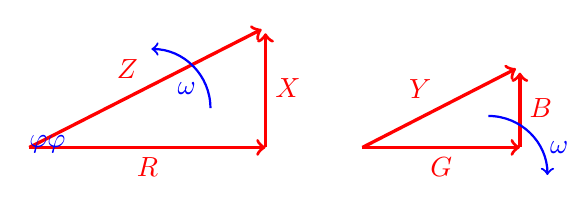
\begin{tikzpicture}


	\coordinate (A1) at (0,0);
	\coordinate (R1) at (3,0);
	\coordinate (X1) at (3, 1.5);
	
	\draw[red, ->, very thick] (0, 0) -- (3, 0);
	\node[red, below] at (1.5, 0) {$R$};
	
	\draw[red, ->, very thick] (3, 0) -- (3, 1.45);
	\node[red, right] at (3, 0.75) {$X$};
	
	\draw[red, ->, very thick] (0, 0) -- (2.95, 1.5);
	\node[red, above left] at (1.5, 0.75) {$Z$};
	
	\draw[blue, ->, thick] (2.3, 0.5) arc (0:90:0.75);
	\node[blue] at (2, 0.75){$\omega$};
	
	\markangle[blue]{X1}{A1}{R1}{$\textcolor{blue}{\varphi}$}{12};
	
	\coordinate (A2) at (4,0);
	\coordinate (R2) at (6,0);
	\coordinate (X2) at (6, 1);
	
	\draw[red, ->, very thick] (4, 0) -- (6, 0);
	\node[red, below] at (5, 0) {$G$};
	
	\draw[red, ->, very thick] (6, 0) -- (6, 0.95);
	\node[red, right] at (6, 0.5) {$B$};
	
	\draw[red, ->, very thick] (4, 0) -- (5.95, 1);
	\node[red, above left] at (5, 0.5) {$Y$};
	
	\draw[blue, ->, thick] (5.6, 0.4) arc (90:0:0.75);
	\node[blue] at (6.5, 0){$\omega$};
	
	\markangle[blue]{X2}{A2}{R2}{$\textcolor{blue}{\varphi}$}{12};
	
	%\HelpCords{0}{0}{8}{3}
\end{tikzpicture}

\end{karte}

\begin{karte}{Was bezeichnet man als Reaktanz?}
	\begin{itemize}
		\item Die Reaktanz ist der Imaginär Teil der Impedanz. Oder auch der Blindwiderstand.
		\item Das Formelzeichen der Reaktanz ist $X$
		\item Für Kapazitäten ist die Reaktanz negativ
		\item Für Induktivitäten positiv
	\end{itemize}
\end{karte}

\begin{karte}{Wie ist die Phasenverschiebung definiert?}
	Die Referenz ist der Strom.\\
	%Autor: Simon Walker
%Version: 1.0
%Datum: 16.12.2019


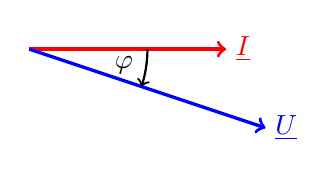
\begin{tikzpicture}
	\coordinate (O) at (0, 0);
	\coordinate (I) at (2.5, 0);
	\coordinate (U) at (3, -1);
	\draw[red, ->, very thick] (O) -- (I);
	\node[right, red] at (I) {$\underline{I}$};
	
	\draw[blue, ->, very thick] (O) -- (U);
	\node[right, blue] at (U) {$\underline{U}$};
		
	\draw[thick, ->] ([shift=(0:1.5cm)]O)  arc[start angle=0, end angle=-18.435,radius=1.5cm];
	
	\node at (1.2, -0.2) {$\varphi$};	
\end{tikzpicture}
\\
	Wenn der Winkel negativ ist (wie im Beispiel) sagt man, dass die Spannung nacheilt, oder der Strom voreilt.
\end{karte}

\begin{karte}{Wie lautet das Ohmsche Gesetz einer Kapazität?}
	\begin{itemize}
		\item $\dfrac{du_{C}}{dt}=\dfrac{i_{C}}{C}$
		\item im Komplexen: $\underline{U} = \dfrac{1}{j \omega C} \cdot \underline{I}$
	\end{itemize}
\end{karte}

\begin{karte}{Was ist die Knotenpotentialmethode}
	\begin{itemize}
		\item Systematische Lösungsmethode
		\item Jeder unabhängige Knoten bekommt eine Gleichung für das Potential
		\item $\mathbf{G} \cdot \vec{u} = \vec{i}$\\
		Leitwertmatrix $\cdot$ Spannungsvektor $=$ Stromvektor
		\item im Komplexen 
		$\mathbf{\underline{Y}} \cdot \underline{\vec{U}} = \underline{\vec{I}}$
	\end{itemize}
\end{karte}

\begin{karte}{Wieso macht ein imaginärer Strom überhaupt Sinn?}
	\begin{itemize}
		\item Er Vereinfacht die Rechnung mit Wechselspannungen
		\item Ein rein imaginärer Strom hat eine Phasenverschiebung von $90^\circ$
	\end{itemize}
\end{karte}

\begin{karte}{Was ist eine elektrische Suszeptanz?}
	\begin{itemize}
		\item Blindleitwert
		\item Der Imaginärteil der Admitanz
		\item Formelzeichen $B$
		\item Positives $B$ $\Rightarrow$ Kapazitive Last
		\item \textcolor{red}{\textbf{Achtung:}} Die Suszeptanz ist nicht der Kehrwert der Reaktanz (Blindwiderstand)
	\end{itemize}
\end{karte}

\begin{karte}{Was bezeichnet man als Scheinleistung?}
	\begin{itemize}
		\item Betrag einer Komplexen Leistung
		\item Produkt zwischen Spannung und Strom\\
		$S=\underline{U}\cdot \underline{I}* = P + jQ$
	\end{itemize}
\end{karte}

\begin{karte}{Warum sind Blindströme oftmals unbeliebt?}
	\begin{itemize}
		\item Die Blindströme fliessen durch die Leitungen und verursachen nur Verluste
	\end{itemize}
	
\end{karte}
